\documentclass[10pt,a4paper]{article}
\usepackage[utf8]{inputenc}
\usepackage{amsmath}
\usepackage{amsfonts}
\usepackage{amssymb}
\usepackage{graphicx}
\usepackage[ngerman]{babel}
\usepackage[a4paper, portrait, margin=1.2in]{geometry}
\author{AW, TS, CS, AD, RB}
\title{Großes Studienprojekt}


\begin{document}
	\maketitle
	\begin{abstract}
		Da IPv4 aufgrund von immer weiter steigenden Nutzerzahlen und internetfähigen Geräte bald nicht mehr als Standardadressraum verwendet werden kann und IPv6 eine mögliche Lösung dieses Problems ist, haben wir uns innerhalb unseres großen Studienprojektes  mit den Aufsetzen und Verwalten eines IPv4 bzw. IPv6 Netzwerkes auseinandergesetzt. 
	\end{abstract}
	\section{Fragestellung}
	Um sich mit dem Zusammenspiel von Geräten innerhalb eines Netzwerkes vertraut zu machen, war gefordert das folgende Diagramm als Netzwerk umzusetzen:
	\begin{figure}[ht]
		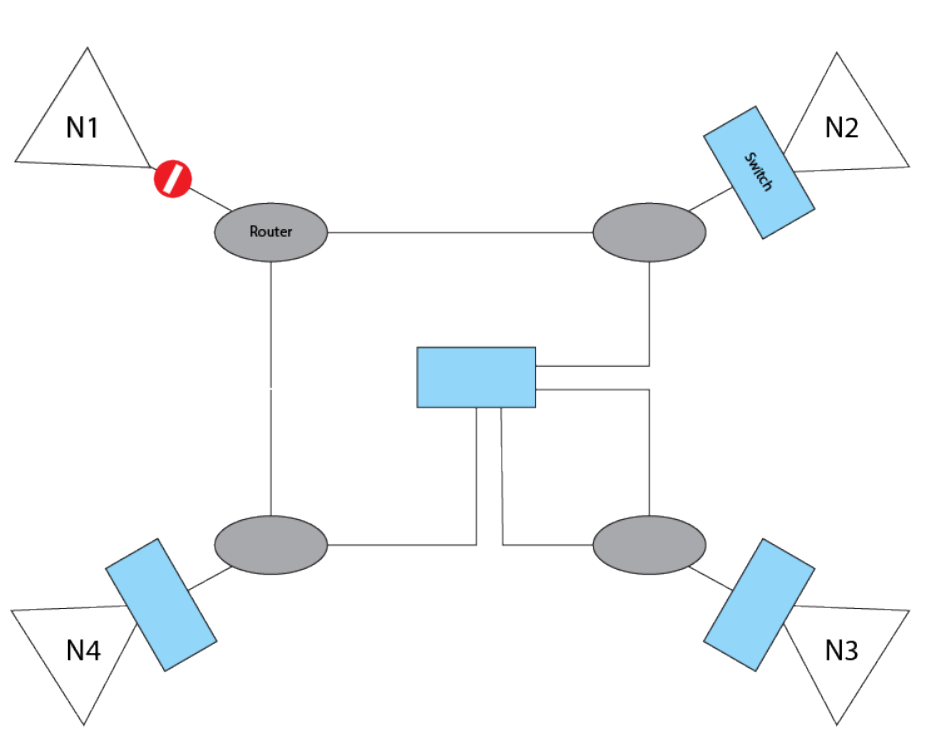
\includegraphics[width=\linewidth]{img/network_topography.png}
		\centering
		\caption{Aufbau des Netzwerks}
	\end{figure}
\par
	Die mit N1 bis N4 beschriftete Dreiecke bezeichnen die von uns aufgestellte Subnetze die durch die Router (graue Ovale, R1 bis R4) aufgebaut werden, und die blaue Vierecke ein Switch. Das \glqq einfahrt Verboten\grqq~ Schild symbolisiert zusätzlich eine von uns konfigurierte Firewall.
\par
	Jeder Router sollte ein eigenen DHCP-Server für das eigene Netzwerk bereitstellen. Alle Router erkennen sich gegenseitig über statische Routes, wobei um zwischen R2 und R4 zu kommunizieren zwei Hops (über R1) benötigt werden. Außerdem werden die Verbindungen zwischen R2 und R3, und R3 und R4 über einem Switch und durch zwei unabhängige VLANs realisiert, die über den Switch in der Mitte konfiguriert werden.
\par
	Hinter R1 ist eine Verbindung zum Internet das durch die Firewall geschützt wird. Die Firewall ist so konfiguriert das sie den ausgehenden Verkehr nicht einschränkt aber nur dann eingehende Pakete weiterleitet wenn sie im Zusammenhang mit einem ausgehenden Paket stehen.
\par
	Der innere Switch sollte zusätzlich so konfiguriert sein das er die Verbindungen zu den Routern über die verbliebene Ports spiegelt.
	
	\section{Herangehensweise}
	Nach ersten Recherchen bezüglich der Router und deren Funktionsweise fiel auf, dass diese auf sehr veralteten Betriebssystemversionen liefen. Deshalb war einer der ersten Arbeitsschritte das Aktualisieren der Firmware. Hiernach ist aufgefallen das in der aktualisierten Version eine GUI zur Verfügung gestellt wurde, mit deren Hilfe jegliche Einstellungen konfiguriert werden konnten. 
\par
	Bevor die Aufgabe bearbeitet wurde war eine Einarbeitung in die Funktionen und Eigenschaften des Systems erforderlich, um eine vollständige Umsetzung der Fragestellung zu realisieren. Dazu wurde ein simples Netzwerk mit Hilfe der Konsole konfiguriert. In diesem Netzwerk wurden alle für die Aufgabenstellung wichtige Komponenten(z.B. DHCP, Firewall, Static Routes, usw.) eingebunden, um ein tieferes Verständnis dieser zu gewinnen.
\par
	Nach ersten Konfigurationen wurde mit Hilfe der GUI geprüft, ob alle Einstellungen erfolgreich übernommen wurden. Dabei ist aufgefallen das mittels der GUI einige Konfigurationen deutlich einfacher und übersichtlicher zu handhaben sind(Bspw. Static Routes). Daher wurde zur Umsetzung der Aufgabenstellung eine Kombination aus Konsole und GUI verwendet.
\par
	Bei der Bearbeitung der Aufgabe musste zu aller erst das Netzwerk auf physischer Ebene, wie auf Abbildung 1 zu sehen, zusammen gesetzt werden. Dabei war eine übersichtliche Verkabelung wichtig, um die Subnetze auch unproblematisch unterscheiden und visualisieren zu können. Des weiteren wurden die Router etikettiert um weitere Übersicht und Organisation zu erschaffen.
\par
	Wichtig war die Dokumentation des Verlaufs der Umsetzung als auch eine Möglichkeit ältere Konfigurationen zu sichern und wieder herzustellen. Hierzu wurde Gitub verwendet, dies erlaubte eine bessere Organisation des Projekts und effektivere Zusammenarbeit.
	
	
	\section{Konfiguration}Christopher
	
	
	\section{Netzwerkanalyse}Rudi
	
	
	\section{Evaluation}Thomas
\end{document}